\documentclass[aspectratio=169]{beamer}

\usetheme{Madrid} % or your favorite theme
\usecolortheme{default}
\setbeamertemplate{footline}[frame number]
% \setbeamertemplate{navigation symbols}{}

\title[]{Extracting lithium from the Salton Sea}
\author[]{Patryk Kozlowski}

\begin{document}

%==================================================
\begin{frame}
  \titlepage
\end{frame}

%==================================================
\begin{frame}{Outline}
  \tableofcontents
\end{frame}

%==================================================
% Add section slides before each section
\AtBeginSection[]{
  \begin{frame}{Outline}
    \tableofcontents[currentsection,hideothersubsections]
  \end{frame}
}

%==================================================
\section{Context on Salton Sea}
\begin{frame}
  \centering
  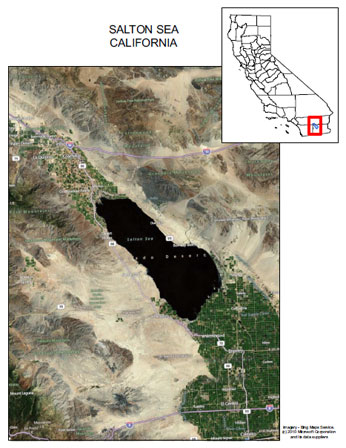
\includegraphics[width=\paperwidth,height=\paperheight,keepaspectratio]{figs/R6_SSea_Right1.jpg}
\end{frame}
\begin{frame}{Historical overview}
\begin{itemize}
  \item Formed when Colorado River breached a levee
\pause
  \item Used to get water due to agricultural runoff
\pause
\item  Now with more rigorous water management due to water stress, sea is drying up
\end{itemize}
\end{frame}
\begin{frame}{Politics}
\begin{itemize}
  \item 1.36 billion dollar loan from Biden administration under CHIPS act
  \pause
  \item Trump canceled the loan, so progress has been slow
\end{itemize}
\end{frame}
\begin{frame}{Environment}
\pause
\begin{itemize}
  \item Has become crucial stopover for migratory birds
  \pause
  \item Regular summer die-offs of fish
  \pause
  \item Study found that children growing up there are 4x more likely to develop asthma
\end{itemize}
\end{frame}
\section{Scientific macroscopics}
\begin{frame}{Elevator pitch}
\begin{figure}
\centering
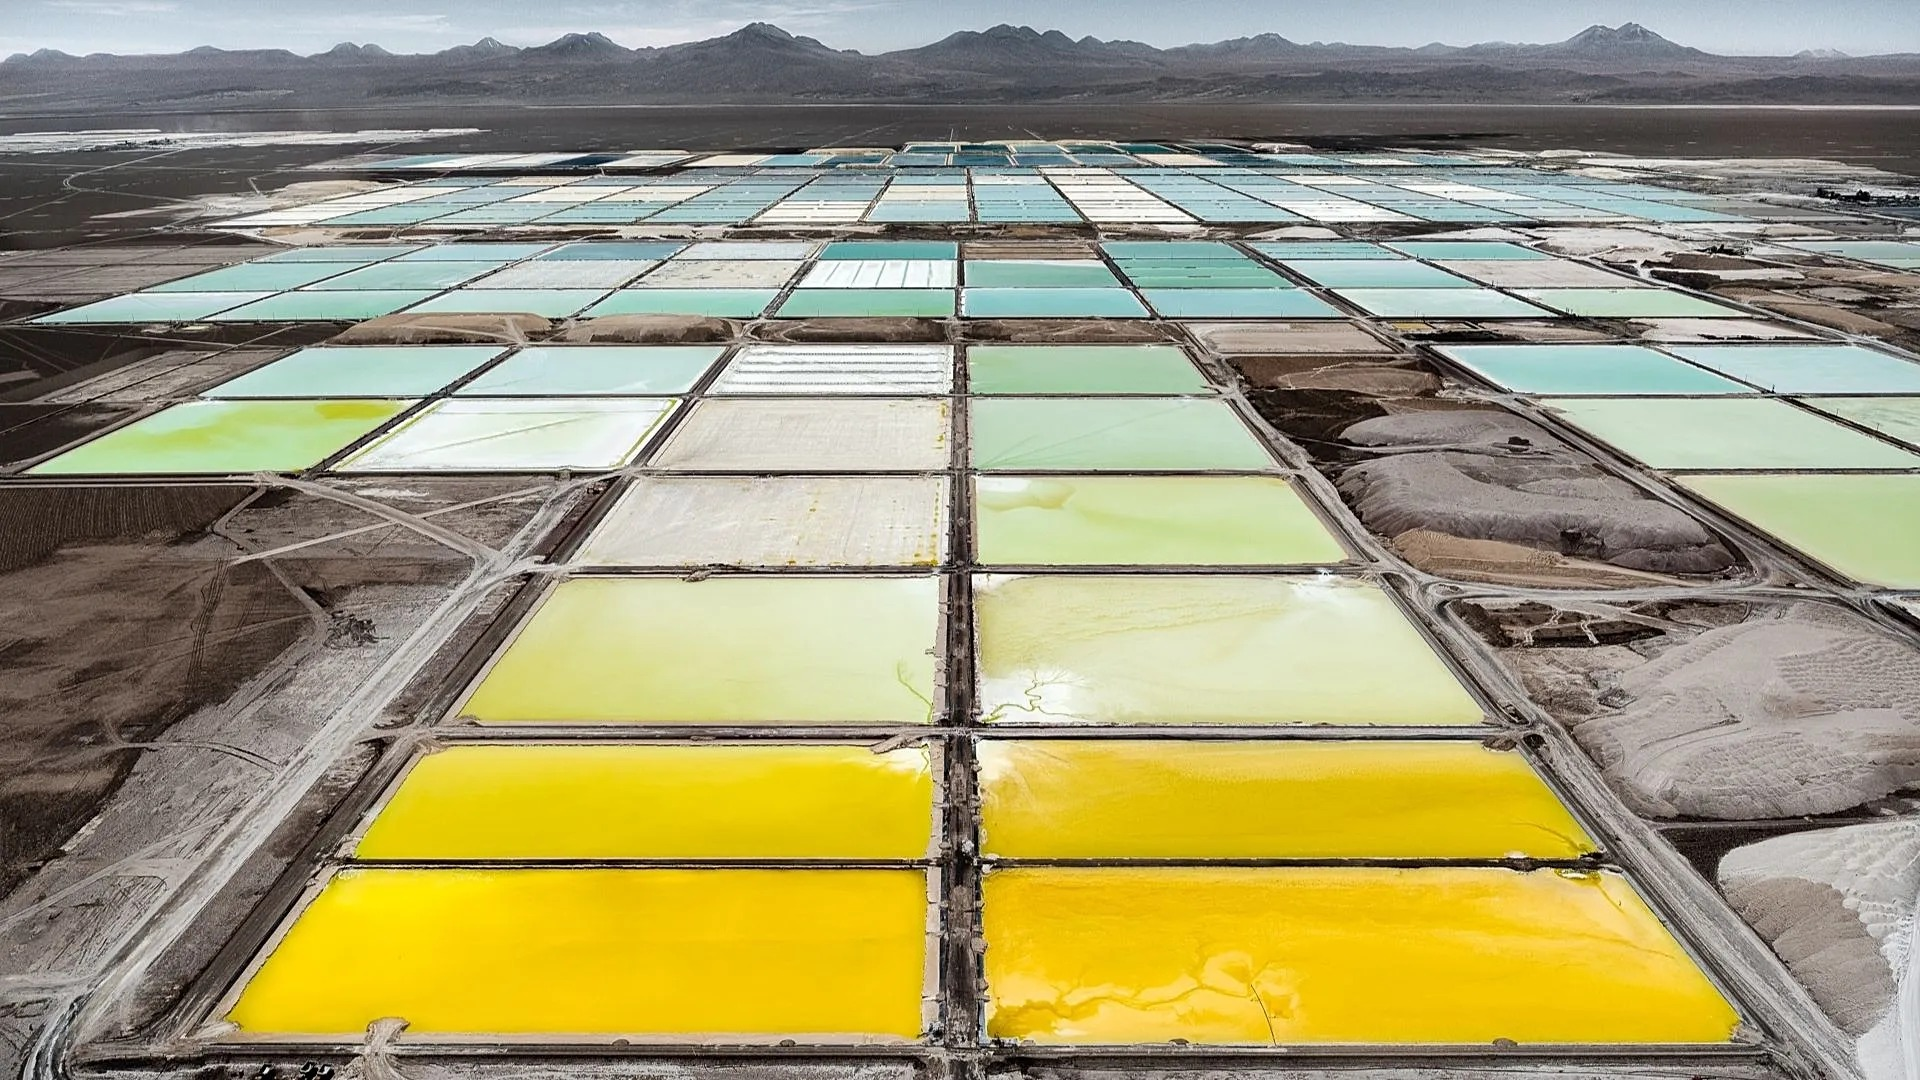
\includegraphics[width=0.5\textwidth]{figs/salt_flats.jpg}
\end{figure}\pause
\begin{itemize}
% \item Conventional lithium mining from brines not suitable for the Imperial Valley
% \item Conventional Li mining from brines relies on solar evaporation followed  by  chemical  precipitation  methods,  which  waste  large amounts of water resources and are not suitable for arid regions like the Salton Sea.
% \item The standard method of extracting lithium involves pumping brine into ponds on the salt flats and processing the lithium salts which crystallise once the water has evaporated. The process requires vast amounts of water.
\item Electro-driven lithium extraction from brines lessens environmental impact\pause
\item Process achieves lithium selectivity over other metal ions.\pause
\item Technoeconomic analysis showed lithium production at one-third of market price% as of January 2023
\end{itemize}
\end{frame}
\begin{frame}{Industrial process}
\begin{figure}
\centering
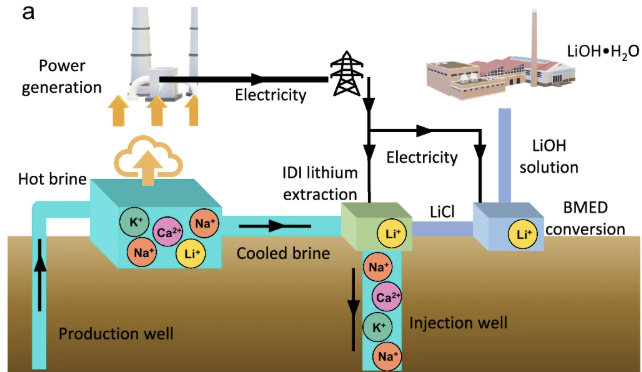
\includegraphics[width=0.8\paperwidth,height=\paperheight,keepaspectratio]{figs/process.png}
\end{figure}
% \begin{itemize}
% \item The entire process
% employs renewable geothermal energy as the sole power input, elim- inating the need for evaporation ponds, fossil fuels, or chemical reagents.
% \end{itemize}
\end{frame}
\begin{frame}{Bipolar membrane electrodialysis}
  \begin{figure}
    \centering
    \begin{minipage}[c]{0.48\textwidth}
      \centering
      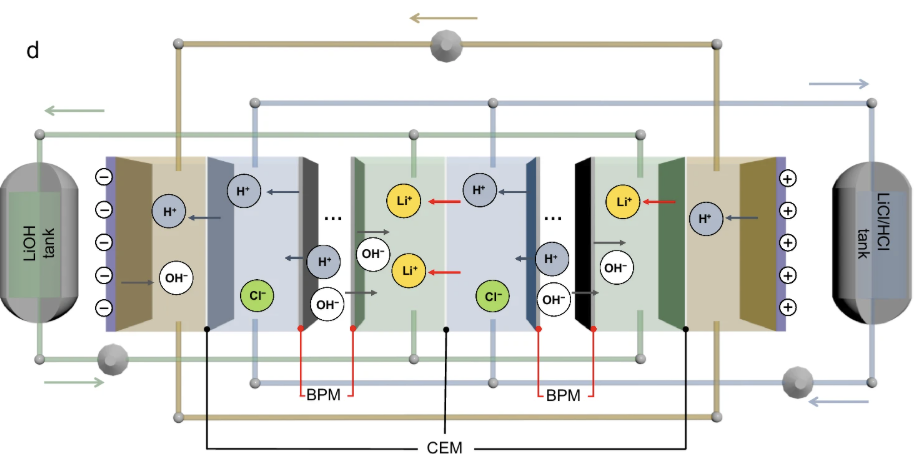
\includegraphics[width=\textwidth,height=0.8\textheight,keepaspectratio]{figs/bmed.png}
      % \caption*{(a) Optional caption}
    \end{minipage}
    \hfill
    \begin{minipage}[c]{0.48\textwidth}
      \centering
      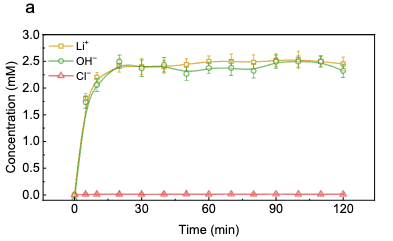
\includegraphics[width=\textwidth,height=0.8\textheight,keepaspectratio]{figs/bmeed_efficacy.png}
      % \caption*{(b) Optional caption}
    \end{minipage}
    % Note the bipolar membrane and then the cation exchange membrane
  \end{figure}
\end{frame}
\begin{frame}{Intercalation deionization}
\begin{figure}
\centering
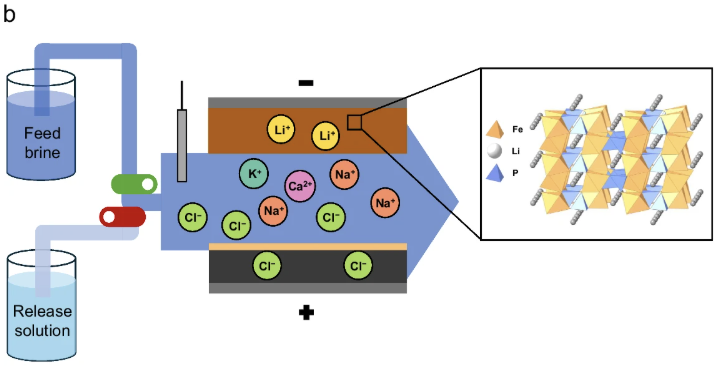
\includegraphics[width=0.8\paperwidth,height=\paperheight,keepaspectratio]{figs/intercalation.png}
% \item Owing to the reversible
% intercalation and deintercalation, lithium intercalation materials can be used for lithium extraction in repeated cycles. During lithiation and delithiation, the electrode potential should be within the water stable window. Salton Sea geothermal brine for lithium extraction has a pH of around 5.514, which sets the water stable window between about 0.5 V versus Ag/AgCl electrode to avoid H
% 2 evolution and 0.7 V versus Ag/ AgCl to avoid O
% 2 evolution
\end{figure}
\end{frame}

\section{Microscopic studies}
\begin{frame}{Intercalation material}
\begin{itemize}
\item Molecular dynamics simulations showed selectivity of LiFePO4 toward Li+
% \item The intrinsic selectivity of LFP toward Li+ has been attributed to its stronger bonding and/or smaller migration barrier than Na+,K+,Mg2+, Ca2+, based on molecular simulations performed in battery systems in the absence of water54
% \item As shown in Fig. 4,Li+ not only exhibits a substantially smaller activation barrier, E
% act =ET
%  EI,defined as the energy gap between the transition and initial states, than any other cations but also solely affords a negative enthalpy change, H
% rxn =EF
%  EI, which is the energy difference between the initial and final states (Table S3). Its small E
% act of 0.063 eV is comparable with the thermal fluctuation energy of k
% bT (i.e., 0.025 eV) at room temperature, making its diffusion nearly dynamically effortless.
\end{itemize}
\begin{figure}
\centering
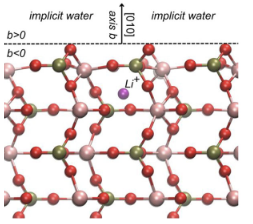
\includegraphics[width=0.5\textwidth]{figs/lifepo4.png}
\end{figure}
\end{frame}
\begin{frame}{DFT study}
\begin{figure}
\centering
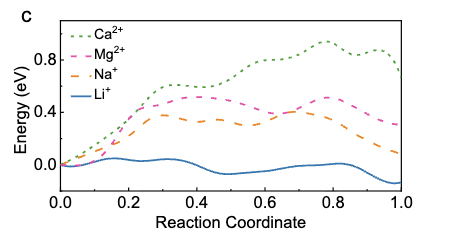
\includegraphics[width=0.75\paperwidth,height=\paperheight,keepaspectratio]{figs/abs_energy.png}
\end{figure}\pause
\begin{itemize}
\item Smaller ion size means better fit in cage\pause
\item Higher valency means greater solvation energy
\end{itemize}
\end{frame}
\begin{frame}{Questions?}
\end{frame}

\end{document}